\chapter{Local Flatness, Geodesics, Rindler Space, and Schwarzschild}

This lecture begins as a continuation, not as a fresh start. We pick up in the middle of a discussion about curvature and flattening, and the thread is worth preserving exactly in that order. First we separate topology from metric choice and from coordinate description. Then we sharpen the local notion of flattening through geodesic coordinates, which leads immediately to the question of where curvature still hides. From there the lecture turns to motion: geodesics, proper time, and the action of a point particle. Only after that groundwork does Susskind insert Rindler space as the model horizon, and only then does he write down the Schwarzschild metric. These notes follow Leonard Susskind's lecture, with the present edition curated with help from LazyingArt LLC and Video2Book.

\section{Topology and Integrated Curvature}

We begin with surfaces, and with a point that is deliberately global. In two dimensions the Gaussian curvature has only one independent component, so one may speak simply of the curvature scalar \(K\). On the standard torus the outer rim has positive curvature, the inner region has negative curvature, and the two balance so that the total curvature vanishes. That is not an accident of the particular drawing. It is a topological statement.

In the lecture's normalization one records the sample values
\begin{align}
\int K\,dA &= +1 && \text{sphere},\\
\int K\,dA &= 0 && \text{torus},\\
\int K\,dA &= -1 && \text{torus with two holes},\\
\int K\,dA &= -2 && \text{torus with three holes}.
\end{align}
We are not proving Gauss--Bonnet here, and the lecture does not try to do so. What matters is the scale of the statement: the integrated curvature depends only on topology. If one puts a bulge on a sphere, or reshapes a torus into a coffee cup, one redistributes positive and negative curvature locally, but one does not change the integral.

That immediately gives the right first distinction. The plane has curvature zero everywhere, and so its integrated curvature is zero. A torus also has zero integrated curvature. A higher-genus surface does not. Therefore a higher-genus surface is topologically ruled out from ever being flattened into a plane. The torus, by contrast, is the only example on the board with any chance. But zero integrated curvature does not prove that a given torus, with its given metric, can be unfolded. It only says that topology does not forbid it.

The lecture then goes one step further: yes, one can put a metric on the torus that is flat everywhere. In other words, the topology of the torus allows an everywhere flat metric even though the familiar embedded doughnut in three-dimensional space is not flat in the metric it inherits from its embedding. This is precisely the separation Susskind wants us to keep in mind: topology constrains, but the metric still matters.

\section{Flattening a Sphere Minus a Point, and Why Bad Maps Do Not Count}

Now suppose we take a sphere and remove one point. Does that produce a torus? No. But can the sphere minus one point be made flat? The lecture answers yes, provided we are willing to abandon the standard round metric. The point is not that the usual sphere is flat. The point is that the sphere minus a point can inherit a different metric, one pulled back from the plane.

The construction is the familiar north-pole projection. Place the sphere tangent to a plane. For any point \(P\) on the sphere, draw the straight line from the north pole through \(P\) and continue it until it reaches the plane. Every point except the north pole is sent to a unique point of the plane.

\begin{figure}[t]
\centering
\begin{tikzpicture}[scale=0.95]
\draw (-3.2,-2) -- (6.0,-2);
\draw (0,0) circle (2);
\fill (0,2) circle (0.05);
\fill (0,-2) circle (0.05);
\fill (1.9,0.62) circle (0.05);
\fill (5.2,-2) circle (0.05);
\draw (0,2) -- (5.2,-2);
\node[above] at (0,2) {$N$};
\node[below] at (0,-2) {$S$};
\node[right] at (1.9,0.62) {$P$};
\node[below] at (5.2,-2) {$P'$};
\node[below left] at (-2.8,-2) {plane};
\node at (0,0) {sphere};
\end{tikzpicture}
\caption{A sphere tangent to a plane, with the north-pole projection used to identify the sphere minus one point with the plane.}
\end{figure}

If we begin with the ordinary flat metric on the plane,
\begin{equation}
ds^2 = dx^2 + dy^2,
\end{equation}
we can pull it back to the sphere minus the north pole. In that pulled-back metric the sphere-minus-a-point is flat. But the lecture insists, correctly, on the price one pays. Points near the north pole map far out on the plane. Therefore neighboring points near the north pole inherit very large distances. The metric components diverge there. So the sphere minus a point can indeed be flattened, but only with a singular metric at the missing point.

This is the right moment for the student's pathological question. Could we not go much further and define a one-to-one map from a square to a line, or from two-dimensional space to one-dimensional space, by interleaving decimal digits? Set-theoretically, yes. One can take two real numbers,
\[
0.a_1a_2a_3\cdots,
\qquad
0.b_1b_2b_3\cdots,
\]
and make a single real number
\[
0.a_1b_1a_2b_2a_3b_3\cdots.
\]
But this is exactly the wrong kind of freedom. Nearby points need not go to nearby points; smooth functions become wildly varying; differentiability is destroyed. As Susskind says, we are not going to regard that as a proper, reasonable coordinate transformation. The lecture uses this digression well: it prunes away the illegitimate notion of flattening and clears the ground for the legitimate local one.

\section{Geodesic Coordinates and Local Curvature}

The right local notion of flattening is geodesic coordinates. We pick a point \(p\) in a curved space. Through \(p\) we draw two perpendicular geodesics and call them, locally, the coordinate axes. For a nearby point \(q\), we assign coordinates by dropping perpendicular geodesics to those axes and measuring the corresponding geodesic distances. The whole construction is only local, but that is exactly the point: we are not trying to flatten the whole manifold, only to flatten the geometry at one chosen point as far as coordinates can do it.

\begin{figure}[t]
\centering

\includegraphics[width=0.74\textwidth]{lecture_11_figure_02.png}
\caption{Blackboard sketch of the local geodesic-coordinate construction at a point.}
\end{figure}

\begin{figure}[t]
\centering
\begin{tikzpicture}[scale=1.0]
\draw (-3.2,0.35) .. controls (-1.8,0.75) and (-0.4,0.55) .. (0.15,0.42)
                     .. controls (1.0,0.22) and (2.0,0.12) .. (3.3,0.45);
\draw (-0.45,-2.6) .. controls (-0.75,-1.2) and (-0.20,-0.2) .. (0.15,0.42)
                    .. controls (0.55,1.0) and (0.85,1.9) .. (1.00,2.75);
\fill (0.15,0.42) circle (0.06);
\draw (0.03,0.42) -- (0.15,0.56) -- (0.27,0.42) -- (0.15,0.28) -- cycle;
\fill (1.55,1.15) circle (0.05);
\draw[dashed] (1.55,1.15) -- (1.08,0.60);
\draw[dashed] (1.55,1.15) -- (0.65,1.55);
\node[below] at (0.15,0.22) {$p$};
\node[right] at (1.62,1.15) {$q$};
\node[below] at (1.15,0.52) {$x$};
\node[left] at (0.75,1.45) {$y$};
\node[below right] at (2.7,0.28) {geodesic axis};
\node[right] at (0.95,2.4) {geodesic axis};
\end{tikzpicture}
\caption{A clean redraw of the local picture: two perpendicular geodesics through \(p\), with nearby coordinates assigned by geodesic distances.}
\end{figure}

In these coordinates the metric tensor at the distinguished point takes its Euclidean form,
\begin{equation}
g_{ij}(p)=\delta_{ij},
\end{equation}
and moreover the first derivatives vanish there,
\begin{equation}
\partial_k g_{ij}(p)=0.
\end{equation}
Since the Christoffel symbols are built from first derivatives of the metric, it follows that
\begin{equation}
\Gamma^{i}{}_{jk}(p)=0.
\end{equation}
This is the precise content of local flatness in the lecture. At one point the metric looks flat, and the first derivative data that would otherwise describe a purely coordinate acceleration has been transformed away.

\subsection{Question \& Answer}

Question: if the Christoffel symbols vanish at the point, why does the curvature not vanish there too?

Answer: because the Riemann tensor has two kinds of terms. Schematically,
\begin{equation}
R \sim \partial \Gamma + \Gamma\Gamma.
\end{equation}
The board writes this schematically, and it is best to preserve that schematic character.

\begin{figure}[t]
\centering

\includegraphics[width=0.62\textwidth]{lecture_11_figure_03.png}
\caption{Blackboard summary: curvature is schematically built from \(\partial\Gamma\) and \(\Gamma\Gamma\), hence from second and first derivatives of the metric.}
\end{figure}

The quadratic \(\Gamma\Gamma\) terms vanish at \(p\), because each Christoffel symbol vanishes there. But the derivative term need not vanish, because it involves derivatives of the Christoffel symbols, and therefore second derivatives of the metric. In the same schematic spirit one may write
\begin{equation}
R \sim \partial^2 g + (\partial g)^2.
\end{equation}
At the chosen point in geodesic coordinates the second term drops out, and what survives is controlled by second derivatives:
\begin{equation}
R(p)\sim \partial^2 g(p).
\end{equation}

This is the invariant lesson the lecture wants to leave with us. By a coordinate choice we can kill first derivatives of the metric at a point. We cannot, in general, kill the second derivatives. The Riemann tensor, the Ricci tensor, and the scalar curvature are therefore tied to that second-derivative data. Curvature is what survives local flattening.

\section{Geodesics, Local Extremality, and the Point-Particle Action}

Once local curvature has been isolated this way, the lecture turns to motion. The point is subtle, and the students push exactly where one should push. A geodesic is not safely defined as the globally shortest path between two points. The official definition, the one that survives all examples, is that the tangent vector is covariantly constant along the curve:
\begin{equation}
u^\nu \nabla_\nu u^\mu = 0,
\qquad
u^\mu=\frac{dx^\mu}{d\tau}.
\end{equation}

\subsection{Question \& Answer}

Question: is a geodesic necessarily a minimum of length, or in spacetime a maximum of proper time?

Answer: only locally, and not always as a minimum. The lecture's example is a high symmetric hill in ordinary two-dimensional space. Between two points on opposite sides there are typically two stable geodesics, one around each side, and also a third path running straight over the summit. That summit path is a geodesic in the official sense, but it is a local maximum of length, not a minimum.

\begin{figure}[t]
\centering
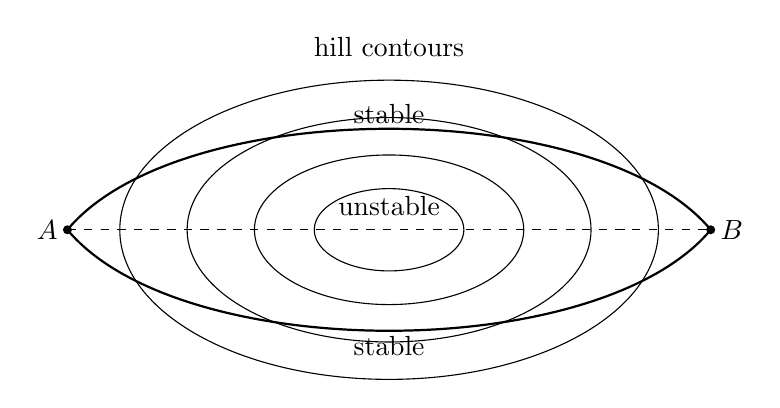
\begin{tikzpicture}[scale=0.95]
\draw (0,0) ellipse (1.0 and 0.55);
\draw (0,0) ellipse (1.8 and 1.0);
\draw (0,0) ellipse (2.7 and 1.5);
\draw (0,0) ellipse (3.6 and 2.0);
\fill (-4.3,0) circle (0.06);
\fill (4.3,0) circle (0.06);
\node[left] at (-4.3,0) {$A$};
\node[right] at (4.3,0) {$B$};
\draw[thick] (-4.3,0) .. controls (-2.8,1.8) and (2.8,1.8) .. (4.3,0);
\draw[thick] (-4.3,0) .. controls (-2.8,-1.8) and (2.8,-1.8) .. (4.3,0);
\draw[dashed] (-4.3,0) .. controls (-1.6,0.0) and (1.6,0.0) .. (4.3,0);
\node at (0,2.45) {hill contours};
\node at (0,0.32) {unstable};
\node at (0,1.55) {stable};
\node at (0,-1.55) {stable};
\end{tikzpicture}
\caption{The hill example from the lecture: two stable side geodesics and one unstable summit geodesic.}
\end{figure}

The string analogy makes the point vividly. If one pulls a string tight between the two points, one stable configuration runs around one side of the hill and another stable configuration around the other. A perfectly symmetric configuration over the summit is also possible, but it is unstable: a tiny displacement makes it slide off. So the lecturer's point is exactly right. ``Geodesic'' and ``minimum distance'' are not identical notions.

From there the lecture pivots to the particle action. By definition, the action of a free point particle moving through spacetime is minus its mass times the proper time along its trajectory:
\begin{equation}
S=-m\int d\tau,
\end{equation}
with
\begin{equation}
d\tau^2=g_{\mu\nu}(x)\,dx^\mu dx^\nu.
\end{equation}
That is not something to derive from a previous principle in this lecture. It is simply the definition of the action.

Now Susskind says, in effect, let us do it. Choose one coordinate, \(x^0=t\), and rewrite the action in terms of coordinate time. The quadratic form becomes
\begin{equation}
g_{\mu\nu}\,dx^\mu dx^\nu
=
g_{00}\,dt^2+2g_{0i}\,dt\,dx^i+g_{ij}\,dx^i dx^j.
\end{equation}
Dividing by \(dt^2\) inside the square root and writing \(\dot x^i = dx^i/dt\), we obtain
\begin{align}
S
&=
-m\int \sqrt{g_{\mu\nu}(x)\,dx^\mu dx^\nu}
\\
&=
-m\int dt\,
\sqrt{g_{00}+2g_{0i}\dot x^i+g_{ij}\dot x^i\dot x^j}.
\end{align}
So the coordinate-time Lagrangian is
\begin{equation}
L(x,\dot x)
=
-m\sqrt{g_{00}+2g_{0i}\dot x^i+g_{ij}\dot x^i\dot x^j}.
\end{equation}

This is a nuisance compared with the ordinary nonrelativistic Lagrangian, because everything sits inside the square root. But conceptually it is the same old machinery: the metric gives a Lagrangian, the Euler--Lagrange equations follow, and one recovers the geodesic equation. The only annoyance, and the lecture explicitly says so, is that the geodesic equation is usually written in terms of \(\tau\), whereas the Euler--Lagrange equations coming from this \(L\) are written in terms of \(t\). One must convert \(d/d\tau\) into \((dt/d\tau)\,d/dt\). It is straightforward but cumbersome, and the lecture quite sensibly refuses to waste the hour on algebraic bookkeeping.

So the result is best stated the way Susskind states it: the principle of stationary proper time and the principle of least action are the same thing in any metric.

\section{Weak Fields and the Role of \texorpdfstring{$g_{00}$}{g00}}

Having obtained the general particle Lagrangian, the lecture pulls it back to the Newtonian regime. This is not a new digression. It is the bridge that reconnects the metric tensor to familiar gravitational physics.

We take the simple case emphasized on the board: only \(g_{00}\) differs appreciably from its flat value, so
\begin{equation}
g_{00}=1+\delta g_{00},
\qquad
g_{0i}=0,
\qquad
g_{ij}\approx -\delta_{ij},
\end{equation}
and we assume the particle velocity is small. Then
\begin{equation}
L \approx -m\sqrt{1+\delta g_{00}-\dot x^{\,2}}.
\end{equation}
Now expand \(\sqrt{1+s}\approx 1+s/2\) for small \(s\). We find
\begin{align}
L
&\approx
-m\left(1+\frac{\delta g_{00}}{2}-\frac{\dot x^{\,2}}{2}\right)
\\
&\approx
-m-\frac{m\,\delta g_{00}}{2}+\frac{m\dot x^{\,2}}{2}.
\end{align}

\begin{figure}[t]
\centering

\includegraphics[width=0.70\textwidth]{lecture_11_figure_05.png}
\caption{Weak-field expansion of the point-particle Lagrangian as it appears on the board.}
\end{figure}

The blackboard progression is worth preserving. The first line is the real expansion. The second line separates it into rest, potential-like, and kinetic pieces. The board shorthand appears to omit an explicit factor of \(m\) in the middle term, but the intended algebra is clear from the first line and from the surrounding discussion.

The kinetic piece is familiar:
\[
\frac12 m\dot x^{\,2}.
\]
The first term is the rest contribution; with \(c\) restored it would become \(-mc^2\) in the Lagrangian. The middle term is the new information. Since the Lagrangian is \(L=T-V\), terms that do not depend on velocity contribute minus the potential energy. So, up to the sign bookkeeping that Susskind freely admits he is handling a bit loosely on the board, the perturbation \(\delta g_{00}/2\) plays the role of the gravitational potential.

The right way to phrase the identification is
\begin{equation}
g_{00}\approx \text{const}+2\Phi.
\end{equation}
Equivalently,
\begin{equation}
\Phi \approx \frac{\delta g_{00}}{2}.
\end{equation}
The reason for the \(\delta\) is important. One does not literally identify \(g_{00}\) with the potential. One identifies its derivatives with the derivatives of the potential, so there is always an additive constant that does not matter physically.

For a point mass the Newtonian potential is
\begin{equation}
\Phi(r)=-\frac{GM}{r}.
\end{equation}
This is exactly the relation the lecture will use in a few minutes when it guesses the \(dt^2\) coefficient of the Schwarzschild metric.

\section{Uniform Acceleration, Rindler Space, and the Horizon Model}

Only now does the lecture return to black holes, and even now it pauses. Before looking at the Schwarzschild metric, Susskind says, it is very important to understand accelerated reference frames in relativity. The reason becomes clear almost immediately: special relativity already gives us a horizon once we use the coordinates of uniformly accelerated observers.

In Newtonian mechanics a uniformly accelerated observer traces a parabola,
\[
x=x_0+v_0 t+\frac12 at^2.
\]
But that cannot be the relativistic answer, because sooner or later such a law produces superluminal motion. The correct uniformly accelerated worldline is a hyperbola:
\begin{equation}
x^2-t^2=R^2.
\end{equation}
This is the first essential point. The second is that a hyperbola of this kind is Lorentz-invariant: Lorentz transformations move points along the same hyperbola, just as rotations move points along a circle. That is why the observer feels the same proper acceleration all along the trajectory.

\begin{figure}[t]
\centering
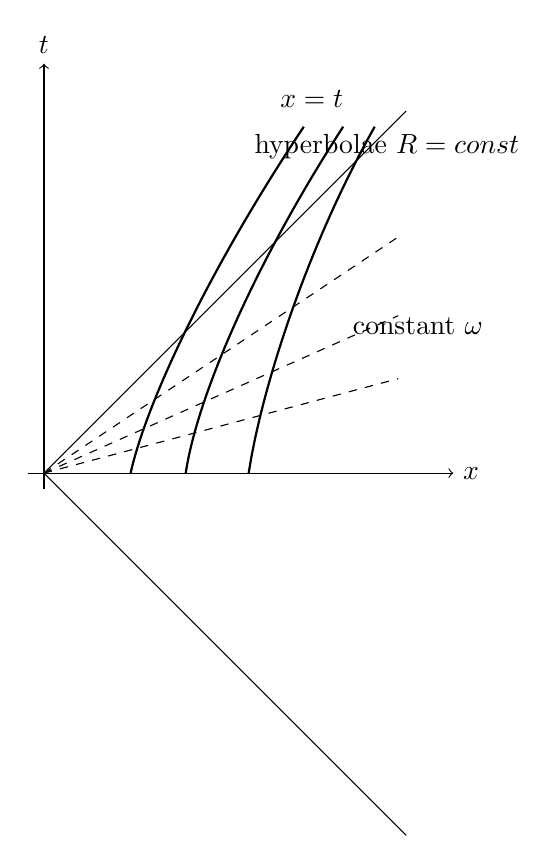
\begin{tikzpicture}[scale=1.0]
\draw[->] (-0.2,0) -- (5.2,0) node[right] {$x$};
\draw[->] (0,-0.2) -- (0,5.2) node[above] {$t$};
\draw[thin] (0,0) -- (4.6,4.6);
\draw[thin] (0,0) -- (4.6,-4.6);
\draw[thick] (1.1,0.0) .. controls (1.3,0.9) and (2.1,2.6) .. (3.3,4.4);
\draw[thick] (1.8,0.0) .. controls (1.95,1.0) and (2.7,2.7) .. (3.8,4.4);
\draw[thick] (2.6,0.0) .. controls (2.75,1.0) and (3.3,2.8) .. (4.2,4.4);
\draw[dashed] (0,0) -- (4.5,1.2);
\draw[dashed] (0,0) -- (4.5,2.0);
\draw[dashed] (0,0) -- (4.5,3.0);
\node at (3.4,4.75) {$x=t$};
\node[below right] at (3.8,2.1) {constant \(\omega\)};
\node[right] at (2.55,4.15) {hyperbolae \(R=\text{const}\)};
\end{tikzpicture}
\caption{The right Rindler wedge of Minkowski space: light cone, hyperbolic worldlines \(R=\text{const}\), and rays of constant Rindler time \(\omega\).}
\end{figure}

A whole accelerated reference frame is made by taking a family of hyperbolae. And here the lecture makes a very important correction to one's Newtonian instincts: a ``uniformly accelerated frame'' does not mean that every observer in the family feels the same acceleration. Quite the opposite. Different members of the family have different proper accelerations. The deeper in one goes toward the origin of the Minkowski diagram, the larger the proper acceleration becomes. In the lecture the scaling is described schematically as \(a\sim 1/R\). That is the closest thing special relativity has to a uniform gravitational field: constant along each trajectory, but not constant from observer to observer.

To coordinatize the right wedge \(x>|t|\), we imitate polar coordinates. Instead of circular functions we use hyperbolic ones:
\begin{equation}
x=R\cosh\omega,
\qquad
t=R\sinh\omega.
\end{equation}
The coordinate \(R\) labels which hyperbola we sit on. The coordinate \(\omega\) runs along the hyperbola and plays the role of time for the accelerated observer. Unlike an ordinary angle, \(\omega\) ranges from \(-\infty\) to \(+\infty\).

Now differentiate:
\begin{align}
dx &= \cosh\omega\,dR + R\sinh\omega\,d\omega,\\
dt &= \sinh\omega\,dR + R\cosh\omega\,d\omega.
\end{align}
Substituting into the flat \(1+1\) dimensional line element,
\begin{equation}
d\tau^2 = dt^2-dx^2,
\end{equation}
we find that the \(dR\,d\omega\) cross terms cancel, and
\begin{align}
d\tau^2
&=
(\sinh^2\omega-\cosh^2\omega)\,dR^2
+
R^2(\cosh^2\omega-\sinh^2\omega)\,d\omega^2
\\
&=
R^2\,d\omega^2-dR^2.
\end{align}
The transverse directions are unchanged by the boost, so the full line element is
\begin{equation}
d\tau^2 = R^2\,d\omega^2 - dR^2 - dy^2 - dz^2.
\end{equation}

This is flat spacetime, but written in accelerated coordinates. The lecture later becomes verbally confused about individual metric components; the clean line element above is the authoritative object. Its physical message is simple: in these coordinates the time-time coefficient grows like \(R^2\), and from the accelerated point of view freely moving objects seem to fall toward \(R=0\). The region \(R>0\) is Rindler space.

\subsection{Question \& Answer}

Question: what does the outside observer see when a rock is dropped, and what does the rock see?

Answer: the rock is inertial. The accelerated observers are not. So in the Minkowski picture the rock moves on a straight worldline, while in the Rindler picture it appears to fall toward the horizon at \(R=0\). But \(R=0\) is not reached at any finite Rindler time. That is the source of the familiar horizon behavior.

\begin{figure}[t]
\centering
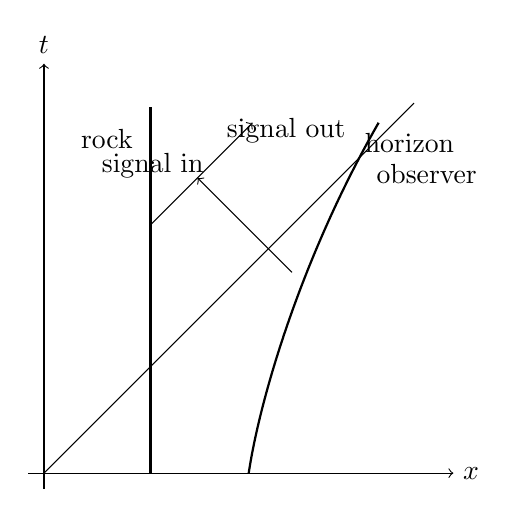
\begin{tikzpicture}[scale=1.0]
\draw[->] (-0.2,0) -- (5.2,0) node[right] {$x$};
\draw[->] (0,-0.2) -- (0,5.2) node[above] {$t$};
\draw[thin] (0,0) -- (4.7,4.7);
\draw[thick] (2.6,0.0) .. controls (2.75,1.0) and (3.3,2.8) .. (4.25,4.45);
\draw[very thick] (1.35,0.0) -- (1.35,4.65);
\draw[->] (3.15,2.55) -- (1.95,3.75);
\draw[->] (1.35,3.15) -- (2.65,4.45);
\node[right] at (4.1,3.8) {observer};
\node[left] at (1.25,4.25) {rock};
\node[above right] at (3.95,3.95) {horizon};
\node[left] at (2.15,3.9) {signal in};
\node[right] at (2.2,4.35) {signal out};
\end{tikzpicture}
\caption{A causal picture of one-way communication across the Rindler horizon. The rock can receive signals from outside, but after crossing the horizon it cannot send signals back out.}
\end{figure}

From the outside observer's point of view, the rock slows down, approaches the horizon asymptotically, and its signals become more and more redshifted. It never quite crosses the horizon in finite \(\omega\). For the falling rock, by contrast, nothing special happens at the crossing. It can continue to receive signals from the outside. The asymmetry is one-way: the rock cannot send information back out once it is behind the horizon. This is why the lecture calls the horizon a kind of one-way door, not a mirror.

The lecture also describes the same motion in the \((R,\omega)\) plane. There the geodesic appears to emerge from \(R=0\) at \(\omega=-\infty\), rise to some maximum value of \(R\), and fall back to \(R=0\) at \(\omega=+\infty\).

\begin{figure}[t]
\centering
\begin{tikzpicture}[scale=0.95]
\draw[->] (-4.4,0) -- (4.4,0) node[right] {$\omega$};
\draw[->] (0,-0.2) -- (0,3.6) node[above] {$R$};
\draw[thick] (-4.0,0.05) .. controls (-2.6,0.45) and (-1.6,2.6) .. (0,2.8)
                         .. controls (1.6,2.6) and (2.6,0.45) .. (4.0,0.05);
\node[below] at (-3.8,0) {$-\infty$};
\node[below] at (3.8,0) {$+\infty$};
\node[left] at (0,2.8) {max \(R\)};
\node[below left] at (-0.15,0.0) {\(R=0\)};
\end{tikzpicture}
\caption{A geodesic in \((R,\omega)\): the horizon lies at \(R=0\), but it is reached only at \(\omega=\pm\infty\).}
\end{figure}

That is the crucial horizon model the lecture wants us to carry forward. Special relativity, written in accelerated coordinates, already teaches us how an outside observer can see a crossing stretched to infinite time while the infalling object experiences nothing dramatic at the horizon.

\section{Flat Spacetime in Spherical Coordinates and the Schwarzschild Metric}

Now we come back to the black-hole problem. The lecture is explicit: we are not going to write down Einstein's equations and solve them by brute force. That is a mess. Instead we will write down the solution in the special case of spherical symmetry, motivate the pieces that can be motivated quickly, and then analyze the geometry.

The first step is to write flat space in coordinates adapted to spherical symmetry. On the unit two-sphere we fix the notation carefully, because the lecture is tired by this point and temporarily flips the symbols. We take \(\phi\) to be the polar angle measured from the north pole, and \(\theta\) the azimuthal angle around the equator. Then
\begin{equation}
d\Omega^2 = d\phi^2+\sin^2\phi\,d\theta^2.
\end{equation}
With this shorthand the metric of flat three-dimensional space in spherical coordinates is
\begin{equation}
ds^2 = dr^2+r^2d\Omega^2,
\end{equation}
and the metric of flat spacetime becomes
\begin{equation}
d\tau^2 = dt^2-dr^2-r^2d\Omega^2.
\end{equation}

This is the natural starting point because the black-hole exterior is spherically symmetric. At that point the lecture inserts Birkhoff's theorem in exactly the limited form needed: outside any bounded spherically symmetric distribution of matter, the metric is the same as the exterior black-hole metric. So the Schwarzschild geometry is the relativistic analogue of the Newtonian point-mass field, though of course the black hole is not particle-like in any naive sense.

Before writing the relativistic answer, Susskind reminds us of the Newtonian one:
\begin{equation}
\Phi(r)=-\frac{GM}{r}.
\end{equation}
And from the earlier weak-field analysis we know that
\begin{equation}
g_{00}\approx \text{const}+2\Phi.
\end{equation}
Asymptotic flatness fixes the constant: very far away from the mass, the geometry must go back to flat spacetime, so the coefficient of \(dt^2\) must tend to \(1\). Therefore the time-time coefficient is led by
\begin{equation}
g_{00}=1-\frac{2GM}{r}.
\end{equation}
The angular part remains exactly what it was in flat space,
\[
-r^2d\Omega^2.
\]
That piece is unaffected by the field equations in this static spherically symmetric case. The hard part, and the part that really does require Einstein's equations, is the radial coefficient. The lecture simply states the result:
\begin{equation}
d\tau^2
=
\left(1-\frac{2GM}{r}\right)dt^2
-
\frac{dr^2}{1-\frac{2GM}{r}}
-
r^2d\Omega^2.
\end{equation}
This is the Schwarzschild exterior metric in units with \(c=1\). If one restores dimensions, the lecture's heuristic dimensional analysis amounts to replacing \(2GM/r\) by \(2GM/(rc^2)\).

Several features of the presentation are worth keeping exactly as they are.

First, the metric is stated and motivated, not derived. That matters. The lecture uses spherical symmetry, asymptotic flatness, and the Newtonian limit to motivate the \(dt^2\) coefficient, and then simply reports the \(dr^2\) coefficient.

Second, the geometry returns to flat spacetime as \(r\to\infty\). This is why ordinary stars do not wildly deform local geometry in everyday circumstances. The dimensionless parameter is really \(GM/(rc^2)\), and the large \(c^2\) in the denominator suppresses the effect unless the source is extremely compact.

Third, the metric looks nothing like the Rindler metric. The lecture ends by stressing exactly that point. The similarity is not supposed to be obvious from the raw formulas. The claim is subtler: the horizon of the Schwarzschild black hole will turn out to be very much like the horizon of Rindler space. That is the next lecture's job.

\section{Summary}

This lecture clears the ground before black holes properly begin. It distinguishes topology from metric choice and from coordinate description; it shows that geodesic coordinates flatten the metric only to first order, leaving curvature behind as second-derivative data; it sharpens the meaning of geodesic so that unstable extremal paths are not excluded by a bad slogan; and it turns proper time into a genuine particle action and hence a Lagrangian.

Then, before writing the Schwarzschild metric, it gives us the simpler horizon of Rindler space. That is the real preparation. In accelerated coordinates flat spacetime already contains an event horizon, already shows one-way communication, and already teaches the difference between what the outside observer sees and what the infalling object experiences. Only after that lesson is in hand does the Schwarzschild metric appear, poised for the next step: to understand the black-hole horizon by comparing it, carefully and locally, to the Rindler horizon.